% !TeX root = RJwrapper.tex
\def\arraystretch{2.5}
\title{\emph{countfitteR}: a package for the analysis of count data}
\author{by Jaros\l{}aw Chilimoniuk, Stefan R\"{o}diger and Micha\l{} Burdukiewicz}

\maketitle

\abstract{
\emph{countfitteR} is a package designed for the analysis of count data and for determination of the most optimal distribution model, since overdispersion has severe impact on data analysis. It comes with easy to use shiny GUI and webserver. Providing clinical scientists simple interface for the analysis of the data, without biostatistical knowledge about nature of distributions. \\
In \emph{countfitteR} we implemented four models of distribution. 
Poisson, which typically is used for count data. Negative Binomial (NB) dealing with extreme values. Zero-Inflated Poisson to depict Poisson-distributed data with excessive zeros. Zero-Inflated Negative Binomial to take care of increased variability of counts and zero-inflation. It can fit counts to mentioned distributions separately or globally, depending on the source of the data.
}

\section{Introduction}
\subsection{Count data, and their prevalence}
Count data is a type of data in which the number of occurrences in a fixed period can take only the non-negative integer values. Examples of count data are found in transportation safety, number of office visits, hospital admissions, adverse drug events (ADEs), laboratory tests, rates of cardiac arrest or infections, and DNA double-strand breaks.

This data is found in injury counts and crash statistics \citep{narayanamoorthy_accommodating_2013, brijs_studying_2008}, clinical trials (e.g., in the context of chronic obstructive pulmonary disease \citep{keene_analysis_2007}).

We developed a system that facilitates the digital  enumeration of DSBs via the phosphorylated histone variant H2AX ($\gamma H2AX$), which is an important  biodositometer during radiation treatment. $\gamma H2AX$ is an important biomarker of physiological and pathological cellular processes \citep{reddig_dna_2018,rodiger_quantification_2018}. Associated biomarkers such as the p53-binding protein 1 (53BP1) may also be detected during the screening. The foci quantification is a fast and sensitive approach for detection of DNA double strand breaks (DSBs).
%, one of 
They are the critical types of DNA damage introduced by radiation, cellular process or toxic agent with applications in research and clinical environment (e.g., individual radiosensitivity). Although these biomarkers play a crucial role in diagnostics, their levels vary not only between patients but also between replicates.

The Poisson distribution is presumably most commonly used when dealing with count data \citep{morina_generalized_2015}. However, in the context of DSBs, real foci data often do not satisfy constraints implied by this distribution. This suggests that another probability distribution for positive integers may describe a data set more accurately. Therefore, an identification of the probability distribution of $\gamma H2AX$ foci and associated biomarkers is vital for the precise estimation of the mean number of foci per cell and its confidence intervals.


\section{Overdispersion}

Overdispersion is an important concept in the analysis of the data. It occurs when the variation is much higher than expected. Usually when this happens we try to fit our dataset to distribution model to get the sample mean as close as possible to population mean \citep{morina_generalized_2015}. Some distribution models have an attribute to fit variabilities of observations.

% Overdispersion may be caused by the increased variability of counts, for example when a counting algorithm under- and overcounts. In such a situation the data might have the NB distribution. The other cause of overdispersion is called zero-inflation and occurs in datasets, where some factor introduced faulty zeros. That means that some counts, regardless of their real state, are treated as zeros. In this case, data has the ZIP distribution. If both faulty zeros and increased variance affect the data, the ZINB distribution is the most appropriate.\\
% Count data is commonly assumed to be Poisson-distributed. One of the important features of the Poisson distribution is the equality of variance and expected value. But often we encounter overdispersed datasets, when the variance is bigger than the mean, and the commonly used model does not have attribute to fit variabilities of observations as close as possible to population mean.\\
% That is why we implemented four distributions in \emph{countfitteR}: Poisson (POIS), Zero-Inflated Poisson (ZIP), Negative Binomial (NB) and Zero-negative Binomial (ZINB) model overdispersed counts.

Most statistical tests developed for determining if data is Poisson-distributed, test the equality of variance and mean. The data is considered overdispersed when the variance is significantly higher than the mean. We consider two possible causes for overdispersion. Firstly, the extreme values (both very high and very low counts) may occur more often than it is assumed in the Poisson distribution. Such situations are well modeled by the negative binomial (NB) distribution. Despite the fact that the NB distribution is used primarily for counting the number of failures before a predetermined number of successes occurs, it can be also alternatively parameterized to describe count data with non-equal variance and mean. One of the important properties of the NB distribution is that the maximum likelihood (ML) estimator of its mean ($\hat{\mu}$) (e.g., the mean number of foci per cell) is equal to the arithmetic mean of counts in a data set.

The second cause of overdispersion is zero-inflation, an excessive number of zeros in a data set. We distinguish two causes for zero-inflation: either zeros occur naturally or false zeros are introduced by an unknown factor (e.g., foci not detected by the system). To describe zero-inflation we use the Zero-Inflated Poisson (ZIP), and the Zero-Inflated Negative Binomial (ZINB) distributions. The former is used to depict Poisson-distributed data, where overdispersion is caused by the excessive zeros, and the latter for data where overdispersion arises from both increased variability of counts and zero-inflation. It is important to note, that in case of zero-inflated distributions, the mean number of counts $\lambda$ is not equal to the average number of foci per cell ($\mu$). To describe their relationship, we need to introduce another parameter, r, which is equal to the fraction of counts faulty turned to zeros. Using the introduced notation: $\lambda = \frac{\mu}{1 - r}$. Henceforth, if we do not correctly identify zero-inflation, we underestimate the real number of foci per cell.

Overdispersed distributions in most cases have variance larger than the Poisson-distributed counts with the same average number of foci per cell ($\lambda$). In consequence, the confidence intervals are wider than in the case of the Poisson distribution. It directly affects the conclusion drawn from a data analysis, because bigger change of the mean number of foci is required, to support the significance of the impact of the treatment. 

Since overdispersion has serve impact on a data analysis, we created \emph{countfitteR} for determination of the count data distribution. Our software fits count data to four distributions, that describe counts: Poisson, NB, ZIP and ZINB. Although statistical tests designed for detecting overdispersion exist, they work properly only in a specific range of values. Furthermore, these tests only indicate if the data is overdispersed, but do not point the suitable probability distribution. Therefore, \emph{countfitteR} selects the most appropriate model using the Bayesian Information Criterion (BIC). The analysis is coupled with an estimation of parameters in the distribution of choice and their confidence intervals.

\section{Models}

In \emph{countfitteR} we have implemented 3 variants of the distribution equations. They are selected according to the specifications of the dataset. %Examples are given below.

Parameters:
\begin{itemize}
\item $\lambda$ - Poisson parameter (average number of foci per cell). 
\item $r$ - zero inflation (fraction of cells treated by system as having no foci regardless of their real state).
\item $\theta$ - dispersion parameter.
\end{itemize}

\subsection{Variant 1}

Usually the NB distribution is parameterized using $\mu$ and $\theta$, but to make comparison clearer, we use $\lambda$ instead of $\mu$. In this parameterization, NB and ZINB are treated as the mixture of Poisson and Gamma ($\Gamma$) distributions.  

\begin{center}
\begin{tabular}{ |c|c| } 
\hline
\bfseries Distribution name & \bfseries pmf \\
\hline
Poisson & $P\{X = k\} = \frac{\lambda^k \exp^{-\lambda}}{k!} $ \\
\hline
Zero-inflated Poisson & $P\{X = k\} = \begin{cases} r + ( 1- r) \exp^{-\lambda},\text{if } k = 0\\ r \frac{\lambda^k \exp^{-\lambda}}{k!},\text{if } k = 1, 2, \ldots \end{cases} $ \\
\hline
Negative Binomial & $P\{X = k\} = \frac{\Gamma (\theta + k)}{\Gamma(\theta) k!}  \left(\left( \frac{\theta}{\theta + \lambda} \right)^\theta \left( \frac{\lambda}{\theta + \lambda} \right) \right)^k$ \\
\hline
Zero-inflated Negative Binomial & $P\{X = k\} = \begin{cases}r + (1 - r) \left( \frac{\theta}{\theta + \lambda} \right)^\theta,\text{if } k = 0\\(1 - r) \frac{\Gamma (\theta + k)}{\Gamma(\theta) k!}  \left(\left( \frac{\theta}{\theta + \lambda} \right)^\theta \left( \frac{\lambda}{\theta + \lambda} \right) \right)^k,\text{if } k = 1, 2, \ldots\end{cases}$ \\
\hline
\end{tabular}
\end{center}

\subsection{Variant 2}

Poisson and Negative Binomial distributions have the same expected value. In case of ZIP and ZINB, the expected value is smaller than the real average number of foci per cell.

% ###################################### change to real average number or leave of foci per cell ?

\begin{center}
\begin{tabular}{ |c|c| } 
\hline
\bfseries Distribution name & \bfseries Expected value \\
\hline
Poisson & $E(X) = \lambda $ \\
\hline
ZIP & $E(X) = (1 - r) \lambda $ \\
\hline
NB & $E(X) = \lambda $ \\
\hline
ZINB & $E(X) = (1 - r)  \lambda $  \\
\hline
\end{tabular}
\end{center}parameterization

\subsection{Variant 3}

Depending on the value of $r$ the variance of ZIP and ZINB may be smaller or bigger than the variance of Poisson distribution. In case of the NB distribution, the variance is always bigger than for the Poisson distribution, although the difference becomes negligible, when the $\theta$ is much bigger than $\lambda^2$.

\begin{center}
\begin{tabular}{ |c|c| } 
\hline
\bfseries Distribution name & \bfseries Variance \\
\hline
Poisson & $\textrm{var}(X) = \lambda $ \\
\hline
ZIP & $\textrm{var}(X) = \lambda (1 - r)(1 + \lambda r)$ \\
\hline
NB & $\textrm{var}(X) = \lambda + \frac{\lambda^2}{\theta} $ \\
\hline
ZINB & $\textrm{var}(X) = (1 - r) \lambda \left( 1 + r\lambda  + \frac{1}{\theta} \right)$ \\
\hline
\end{tabular}
\end{center}


\section{2. \emph{countfitteR package}}

%\section{Describe briefly main functions}

\emph{countfitteR} provides clinical scientists with a simple interface for the analysis of count data regardless of their biostatistical knowledge about the nature of the distribution. The framework covers two most common situations. In the first approach, each count is separately fitted to all above mentioned distributions. This is preferable for situations, where counts come from various sources. The second approach relies on fitting globally all counts to a distribution. Such a model is appropriate among others for technical replicates.
Our software is open source and accessible also from the command-line level. It is suitable for integration into other analysis pipelines dealing with count data. Therefore, we anticipate that our finding will have a broader use. 
The web server is accessible under: 
\url{update me}
% #############################################################################3 add web server url

\section{Data sets}
In the present study we used count data from an image based study of $\gamma H2AX$ foci. The data was generated from human peripheral blood mononuclear cells (PBMCs) which were treated with the topoisomerase inhibitor etoposide to induce $\gamma H2AX$ foci. Analysis of such foci data is a common task both in life sciences and in diagnostics applications. \emph{countfitteR} was initially developed for modeling count data from the AKLIDES system \citep{willitzki_fully_2013}. As recently presented in a review \citep{schneider_open_2019}, it can be used for foci data from other bioimage informatics systems.
The data were prepared as described in \citep{rodiger_quantification_2018}. The Comprehensive R Archive Network (CRAN), which archives R packages, has a recommended size limit of five megabytes (MB) \citep{anderson_hosting_2017}. Therefore, the following data sets are included only.

\newpage

{\bfseries
\begin{example}
>foci_count[1:15, 1:5]
\end{example}
}

\scriptsize{
\begin{example}
   L3_AF_DMSO_B_10_FITC L3_AF_DMSO_B_10_APC L3_AF_100_ETP_11_FITC L3_AF_100_ETP_11_APC L3_AF_100_ETP_12_FITC
1                     0                   0                     0                    0                     0
2                     0                   0                     0                    1                    19
3                     0                   0                     0                    0                     0
4                     0                   0                     1                    0                    12
5                     0                   0                     0                    0                     4
6                     0                   0                    13                    0                     1
7                     0                   0                     0                    0                     0
8                     0                   0                     0                    0                     3
9                     0                   0                     0                    0                     8
10                    0                   0                    12                    0                     0
11                    0                   0                     5                    0                     0
12                    0                   0                    21                    0                     0
13                    0                   0                     0                    0                     0
14                    0                   0                     0                    0                     0
15                    0                   0                     0                    0                    11
\end{example}
}

The data of human PBMCs was taken from a study, which showed that freezing and thawing of PBMCs does not significantly influence of $\gamma H2AX$ foci formation \citep{ruhe_effect_2018}. However, the results of this experiment where statistically analyzed using \emph{Prism} (GraphPad Prism Inc.).

\section{Shiny GUI} %Graphical User Interface

Our application is available as a web server that may be used in an analysis of any kind count data, not only $\gamma H2AX$ and 53BP1. An in-depth manual depicts the implemented framework and a rationale behind it. The guide covers both theoretical fundamentals and usage of \emph{countfitteR}, from a data import to a report generation.

If the web server is down or access to the Internet is restricted, access to the package’s capabilities is done by using the command in the R console. It initiates a graphical user interface (GUI), which starts a shiny server on a local PC, it runs as long as the window is open (Figure \ref{fig_gui}). This mode can be named “server-less mode”, as it does not require an external server to run.

\begin{figure}[htbp]
  \centering
  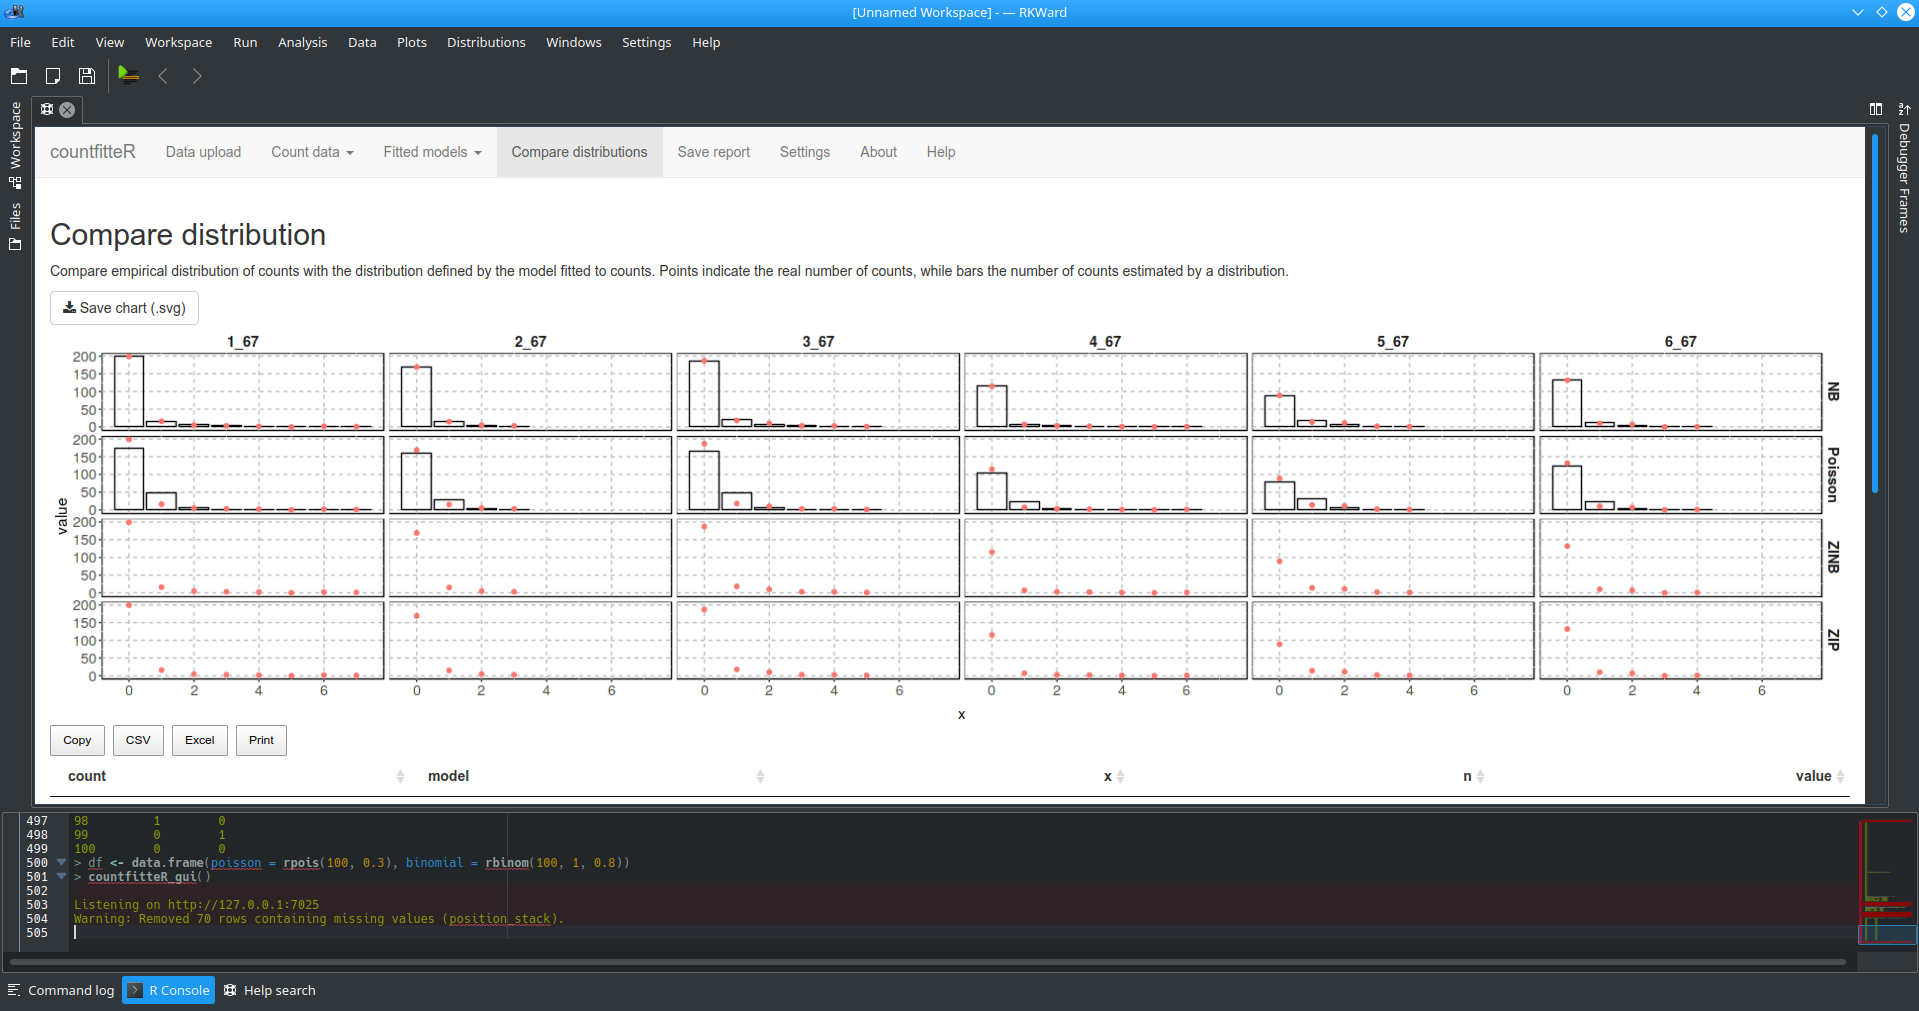
\includegraphics[width=0.99\columnwidth]{fig_gui}
  \caption{\emph{countfitteR\_gui()} function running in the \emph{RKWard} GUI/IDE (v. 0.7.0z+0.7.1+devel1) on Kubuntu 18.04. \citep{rodiger_rkward:_2012}.}
  \label{fig_gui}
\end{figure}
In \textit{Data upload} tab the csv file with count data can be uploaded (Figure \ref{cf_main}). But before that one of csv separators types must be selected to properly load file. If the data file does not have a header the box should be unchecked. If no file will be uploaded, example file will be loaded.

\begin{figure}[htbp]
  \centering
  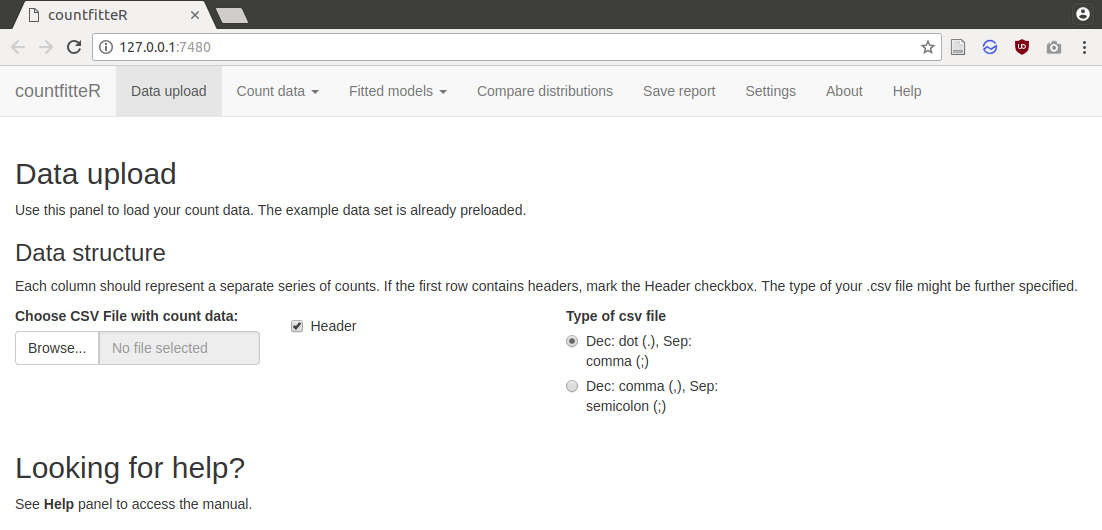
\includegraphics[width=0.99\columnwidth]{fig/cf_main.png}
  \caption{Starting page of the \emph{countfitteR} shiny GUI, where user can upload their data.}
    \label{cf_main}
\end{figure}

In \textit{Count data} tab there are 3 submenus. \textit{Edit input data}, where the loaded data can be reviewed and modified (addition and removal of values and rows) if needed (Figure \ref{cf_cd1}). However, changes will not be tracked and reported in the summary. \textit{Summary} summarizes statistics of data in table (Figure \ref{cf_cd2}). In \textit{Distribution} menu the distribution of counts are displayed in form of barplots or table (Figure \ref{cf_cd3}).

\begin{figure}[htbp]
  \centering
  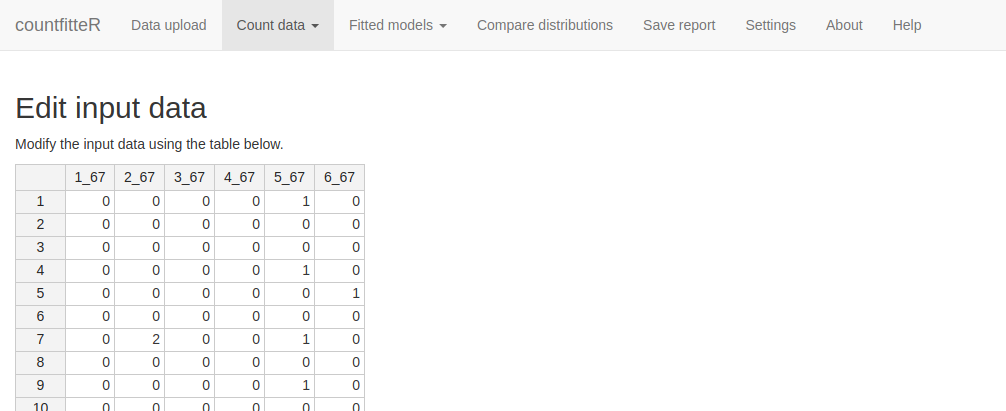
\includegraphics[width=0.99\columnwidth]{fig/cf_cd1.png}
  \caption{In this section uploaded data can be previewed and modified.}
    \label{cf_cd1}
\end{figure}

\begin{figure}[htbp]
  \centering
  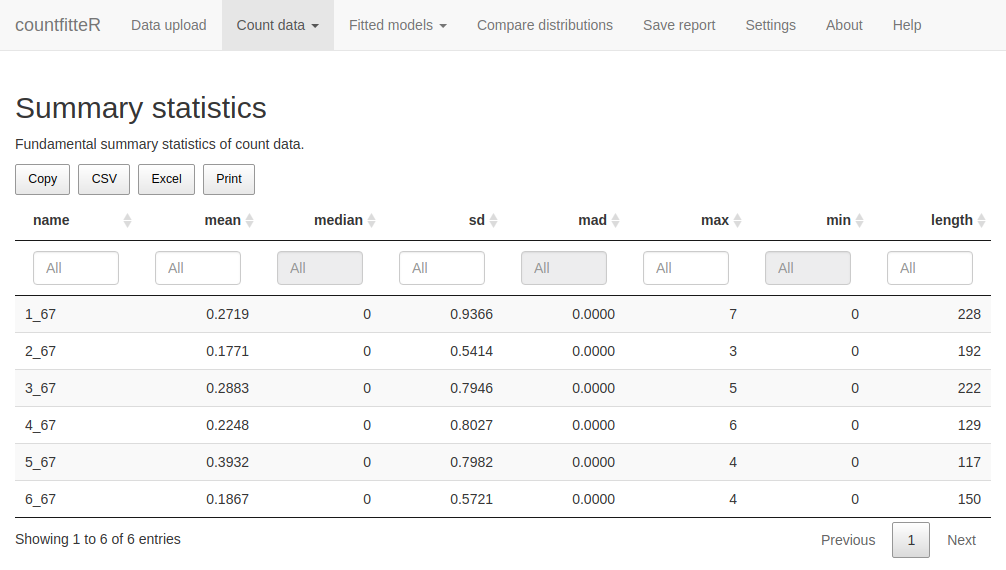
\includegraphics[width=0.99\columnwidth]{fig/cf_cd2.png}
  \caption{Table shows summary statistics calculated for each count.}
    \label{cf_cd2}
\end{figure}

\begin{figure}[htbp]
  \centering
  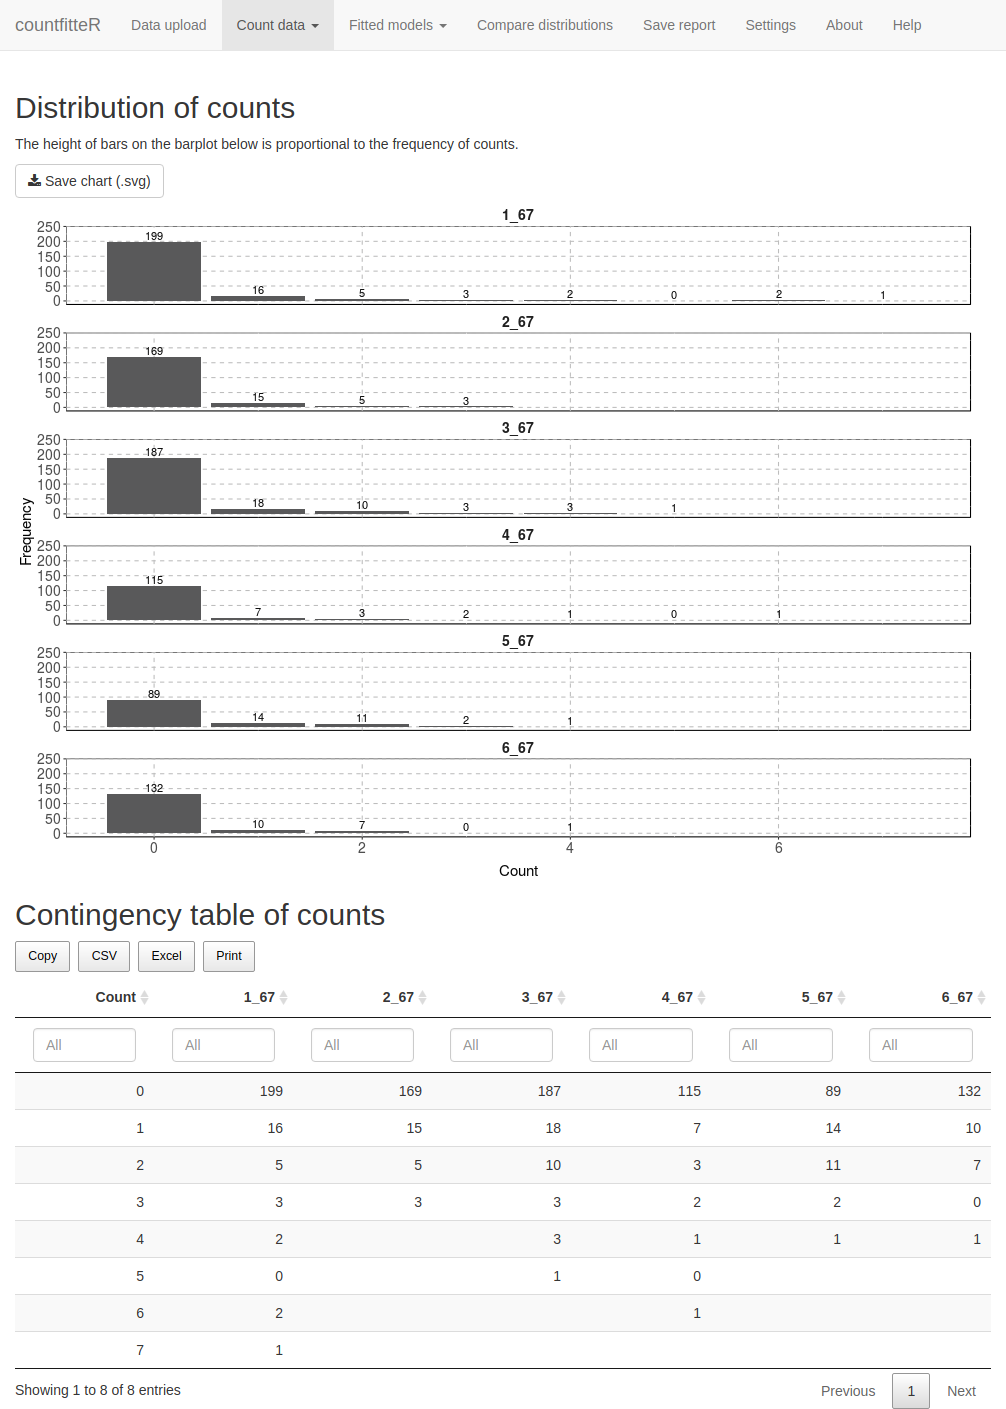
\includegraphics[width=0.99\columnwidth]{fig/cf_cd3.png}
  \caption{Distribution of counts can be viewed in form of a plot or table.}
    \label{cf_cd3}
\end{figure}

Another tab is \textit{Fitted models}. In \textit{Mean value estimate} submenu the mean value estimates, and their confidence are displayed on the plots. Below table with summary of estimates, along with the BIC values of their models can be found (Figure \ref{cf_fm1}). The table in \textit{Coefficients} shows estimated coefficients of models (Figure \ref{cf_fm2}). The \emph{countfitteR} selects the most optimal distribution model for each count, decision can be viewed in the \textit{Decision} submenu (Figure \ref{cf_fm3}).

\begin{figure}[htbp]
  \centering
  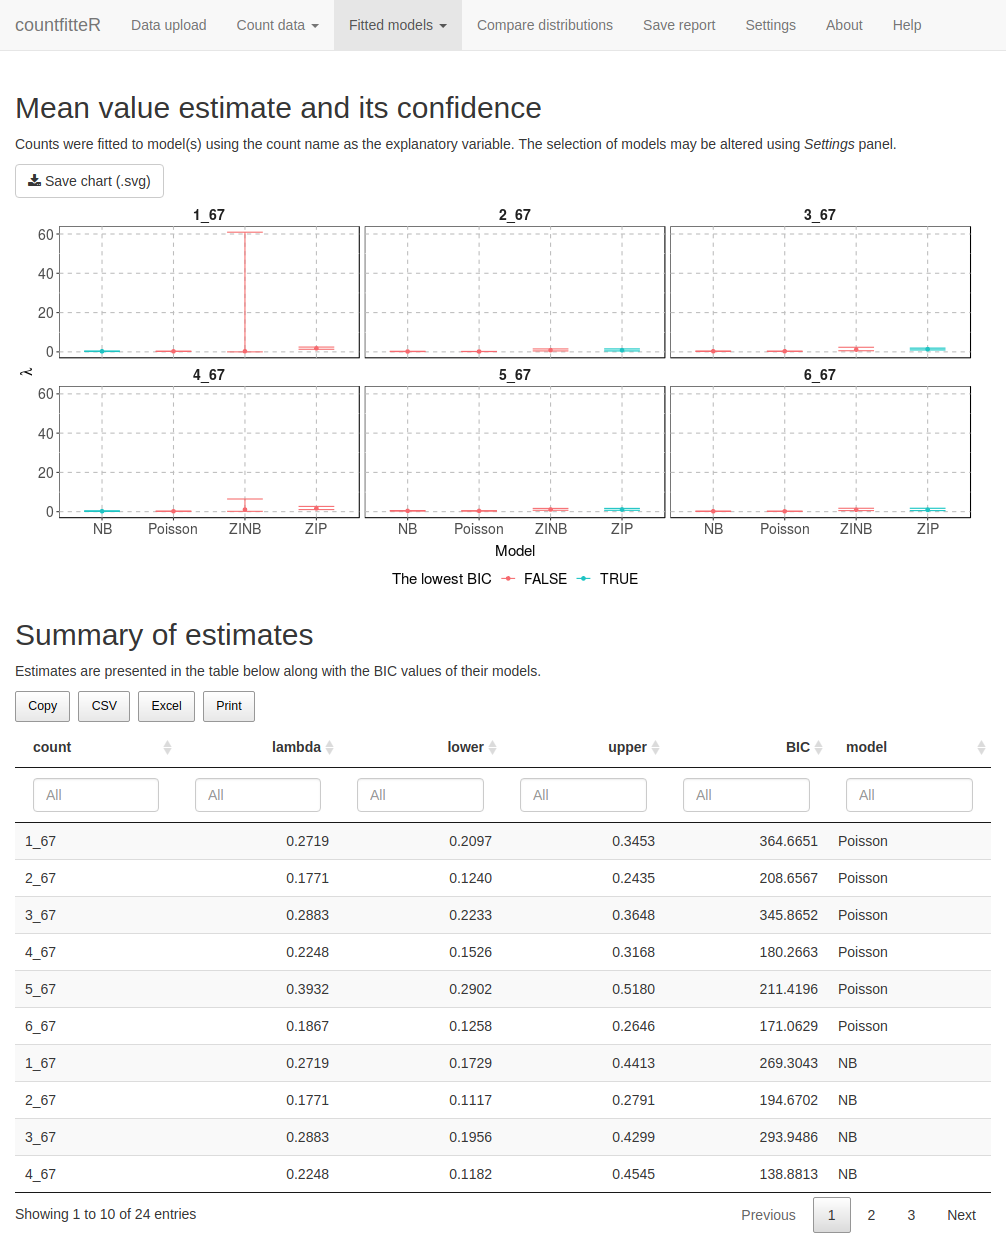
\includegraphics[width=0.99\columnwidth]{fig/cf_fm1.png}
  \caption{Plot and a table shows estimated mean value and its confidence.}
    \label{cf_fm1}
\end{figure}

\begin{figure}[htbp]
  \centering
  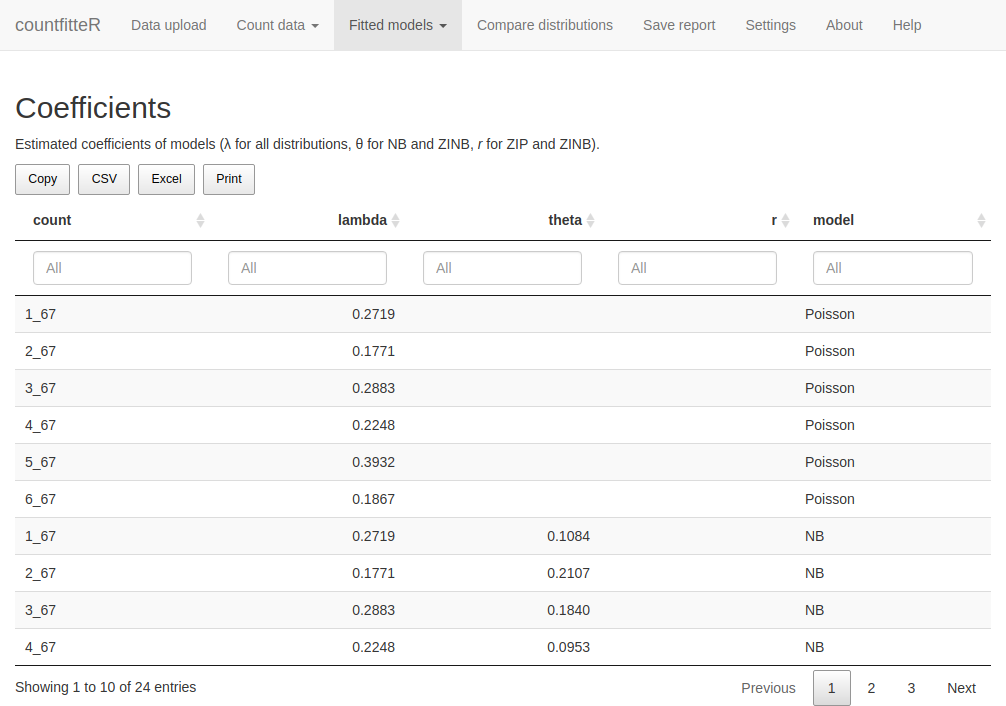
\includegraphics[width=0.99\columnwidth]{fig/cf_fm2.png}
  \caption{Estimated coefficients values of distribution models.}
    \label{cf_fm2}
\end{figure}

\begin{figure}[htbp]
  \centering
  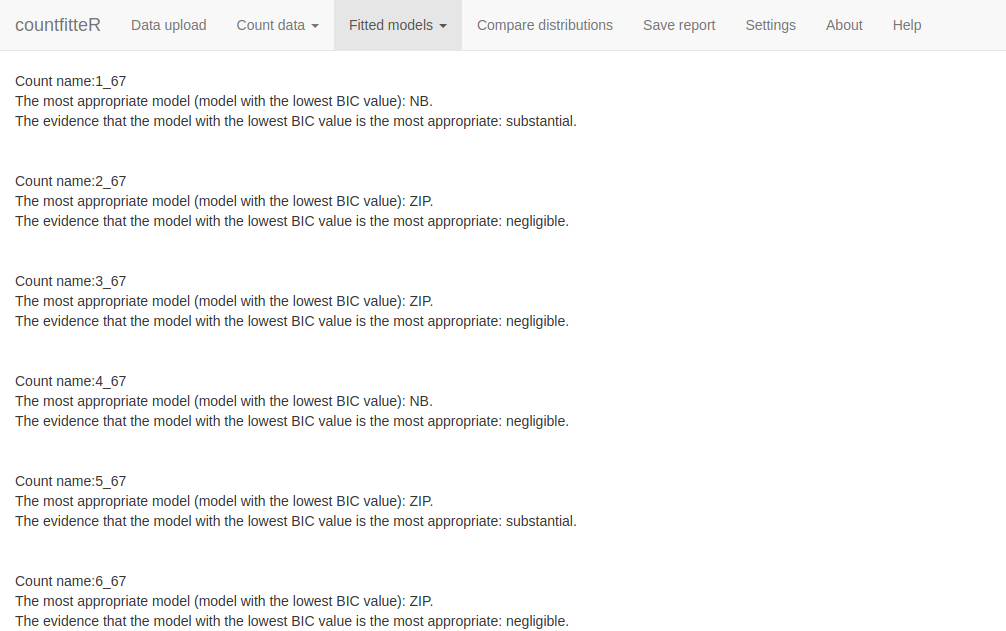
\includegraphics[width=0.99\columnwidth]{fig/cf_fm3.png}
  \caption{\emph{countfitteR} decides on the most optimal distribution model.}
    \label{cf_fm3}
\end{figure}

\textit{Compare distributions} tab shows plots with compared empirical distributions of counts, defined by the model fitted to counts. Red points indicate the real number of counts, while bars represents the number of counts estimated by a distribution model (Figure \ref{cf_cmp}).

\begin{figure}[htbp]
  \centering
  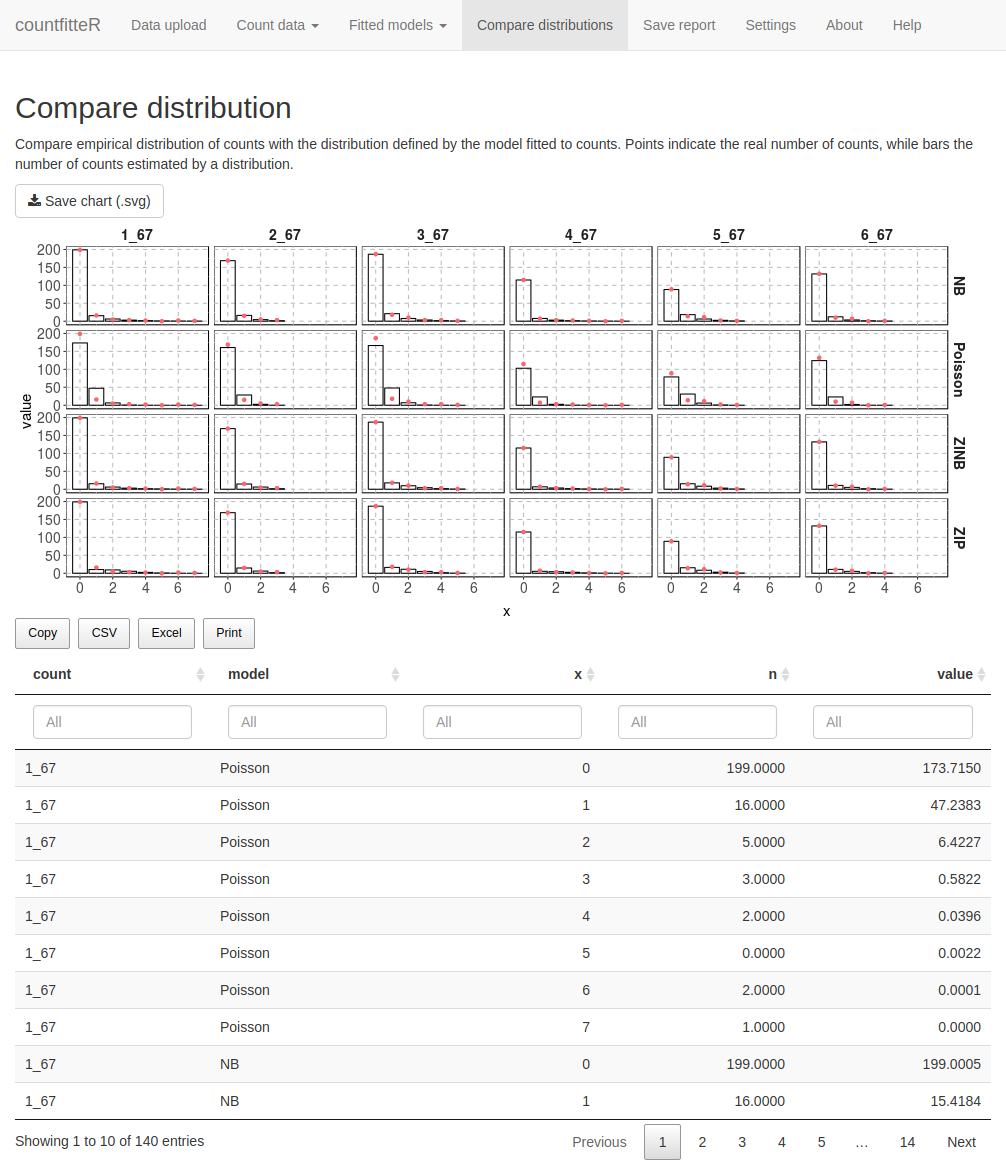
\includegraphics[width=0.99\columnwidth]{fig/cf_cmp.png}
  \caption{Comparison of empirical distribution of counts with distribution models.}
    \label{cf_cmp}
\end{figure}

Other tabs are \textit{Save report}, where all the results, obtained from functions described above, can be saved in one file. All reports are properly created only by opening shiny gui in web browser (Figure \ref{cj_rep}). In \textit{Settings} by default all 4 distribution models are selected for the analyses. The confidence level can be modified and if the \textit{Separate experiment} is marked it assumes that all counts may come from different distributions (Figure \ref{cj_set}). In \textit{About} tab authors and link to repository of \emph{countfitteR} is found and \textit{Help} there features general tips for each tab. 

\begin{figure}[htbp]
  \centering
  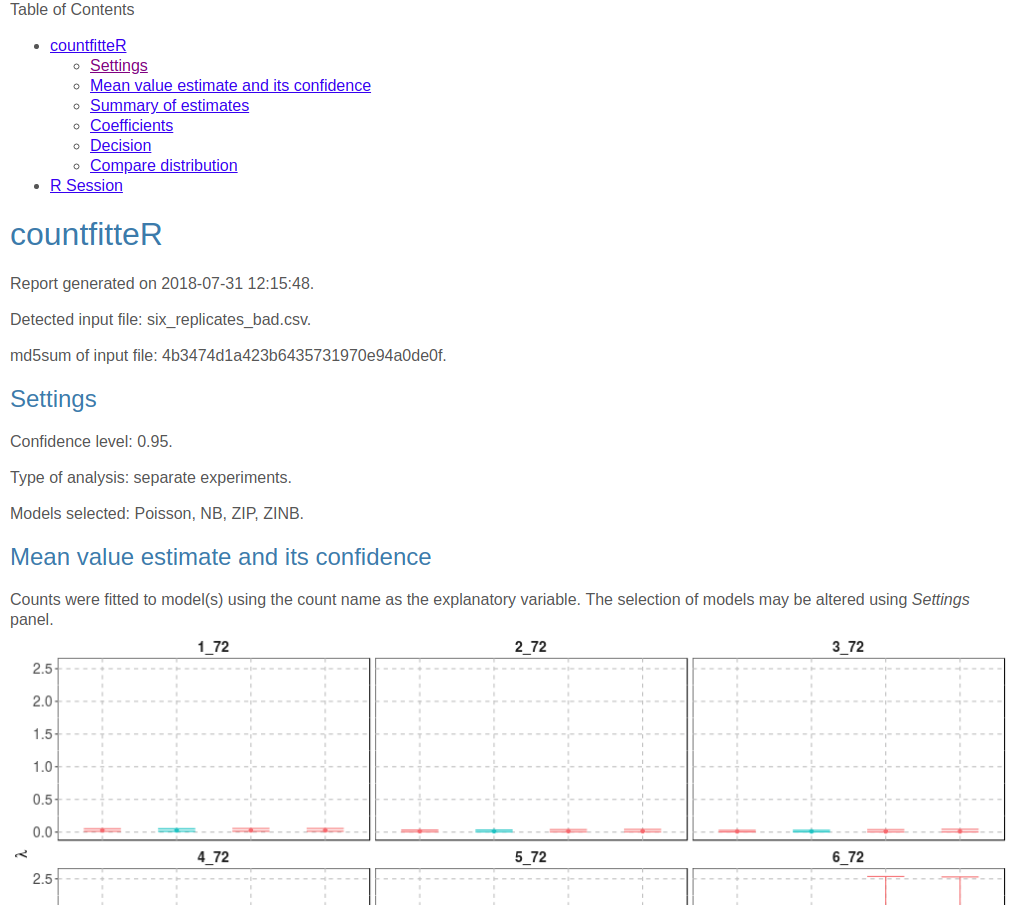
\includegraphics[width=0.99\columnwidth]{fig/cf_rep.png}
  \caption{Fragment of report generated by \emph{countfitteR}.}
  \label{cf_rep}
\end{figure}

\begin{figure}[htbp]
  \centering
  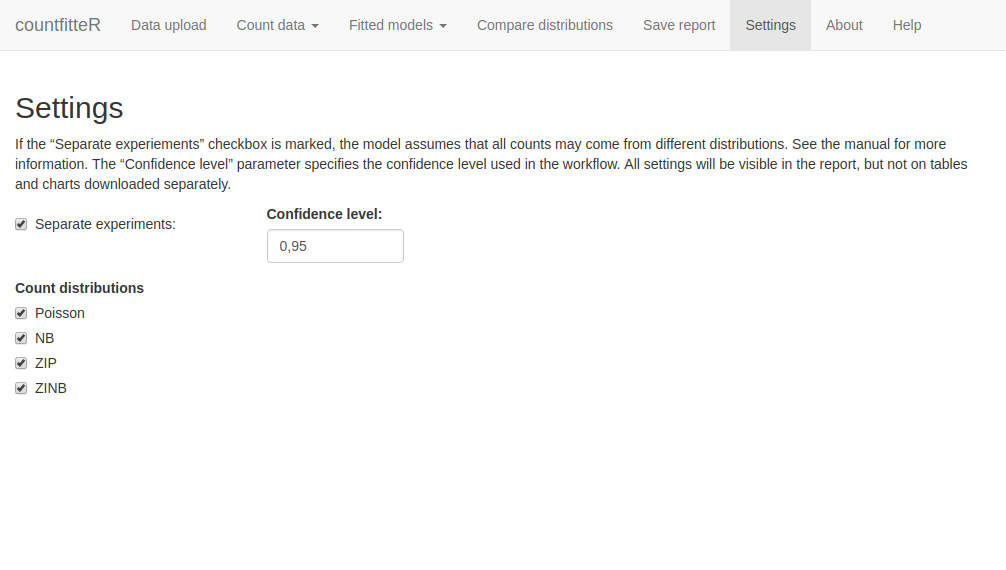
\includegraphics[width=0.99\columnwidth]{fig/cf_set.png}
  \caption{Options in settings menu.}
  \label{cj_set}
\end{figure}

All plots can be saved in svg files and tables in csv.

The graphical user interface  (GUI) was created using  the shiny package \citep{shiny}. This allows \emph{countfitteR} to run as a web server, which can be used on a web browser on any personal computer. The software relies on several packages including \emph{ggplot2} \citep{ggplot2}, \emph{MASS} \citep{MASS}, \emph{stats}, \emph{tools} \citep{Rrr}, \emph{shinythemes} \citep{shinythemes}, \emph{rhandsontable} \citep{rhandsontable}, \emph{pscl} \citep{pscl}, \emph{DT} \citep{DT}, \emph{rmarkdown} \citep{rmarkdown}, \emph{reshape2} \citep{reshape2}, \emph{grid} \citep{Rrr}, \emph{gridExtra} \citep{gridextra} and \emph{dplyr}  \citep{dplyr}.


% \begin{figure}[htbp]
%   \centering
%   \includegraphics[width=0.99\columnwidth]{cj_main}
%   \caption{EXAMPLE \emph{countfitteR} shiny app running in the \emph{R Studio} GUI/IDE \citep{}.}
%   \label{figure:cj_m.png}
% \end{figure}
% 
% \begin{figure}[htbp]
%   \centering
%   \includegraphics[width=0.99\columnwidth]{cj_cmp}
%   \caption{EXAMPLE \emph{countfitteR} shiny app running in the \emph{R Studio} GUI/IDE \citep{}.}
%   \label{figure:cj_cmp.png}
% \end{figure}

\section{Functions that can be used from the command line}

\begin{itemize}
    \item \textit{fit\_counts} - fits counts to distribution models and creates a list of parameters characterizing chosen distribution model.

{\bfseries
\begin{example}
> df <- data.frame(poisson = rpois(25, 0.3), binomial = rbinom(25, 1, 0.8))
> fc <- fit_counts(df, model = "pois") 
\end{example}
}

\begin{example}
$poissonpois
$poissonpois$coefficients
lambda 
  0.28 

$poissonpois$confint
          lower     upper
lambda 0.120304 0.5414518

$poissonpois$BIC
[1] 35.0404

$poissonpois$model
[1] "pois"


$binomialpois
$binomialpois$coefficients
lambda 
  0.64 

$binomialpois$confint
           lower    upper
lambda 0.3753717 1.006709

$binomialpois$BIC
[1] 49.50006

$binomialpois$model
[1] "pois"
\end{example}


    \item \textit{compare\_fit} - compares empirical distribution of counts with the distribution defined by the model fitted to counts. Creates data table with distribution values for each unique count.


{\bfseries
\begin{example}
> df <- data.frame(poisson = rpois(25, 0.3), binomial = rbinom(25, 1, 0.8))
> cmp <- compare_fit(df, fitlist = fit_counts(df, model = "all"))
\end{example}
}

\begin{example}
      count   model x  n     value
1   poisson Poisson 0 18 18.894594
2   poisson Poisson 1  7  5.290486
3   poisson     ZIP 0 18 18.894681
4   poisson     ZIP 1  7  5.290388
...
13 binomial      NB 0  9 13.182392
14 binomial      NB 1 16  8.436568
15 binomial    ZINB 0  9 13.182335
16 binomial    ZINB 1 16  8.436642
\end{example}

    \item \textit{plot\_fitcmp} - creates plot from compare\_fit results. The bar charts represent theoretical counts depending on the chosen distribution. Red dots describe the real number of counts.

{\bfseries
\begin{example}
> df <- data.frame(poisson = rpois(25, 0.3), binomial = rbinom(25, 1, 0.8))
> cmp <- compare_fit(df, fitlist = fit_counts(df, model = "all"))
> plot_fitcmp(cmp)
\end{example}
}

\begin{figure}[htbp]
  \centering
  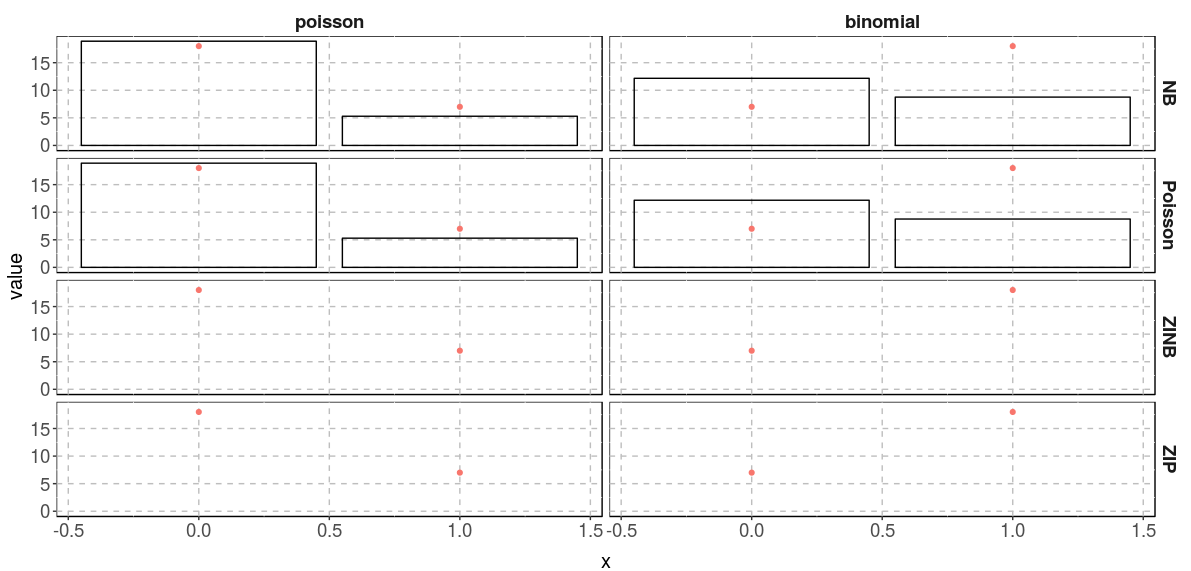
\includegraphics[width=0.99\columnwidth]{Rplot}
  \label{figure:Rplot.png}
\end{figure}

\item \textit{summary\_fitlist()} - creates data frame from a list created by \textit{fit\_counts()} function with additional attributes. Data frame with summarized results of all distribution models.

{\bfseries
\begin{example}
> df <- data.frame(poisson = rpois(25, 0.3), binomial = rbinom(25, 1, 0.8))
> fc <- fit_counts(df, model = "all")
> summary_fitlist(fc) 
\end{example}
}
% \footnotesize
\scriptsize{
\begin{example}
                 count    lambda     lower     upper      BIC      theta            r   model
poisson_pois   poisson 0.2800000 0.1203040 0.5414518 35.04040         NA           NA Poisson
binomial_pois binomial 0.6400000 0.3753717 1.0067089 49.50006         NA           NA Poisson
poisson_zip    poisson 0.2800081 0.1334780 0.5873969 38.25936         NA 3.943333e-05     ZIP
binomial_zip  binomial 0.6400005 0.3920834 1.0446771 52.71905         NA 6.847516e-06     ZIP
poisson_nb     poisson 0.2800000 0.1203060 0.5414187 38.25952   7869.428           NA      NB
binomial_nb   binomial 0.6400000 0.3753665 1.0067211 52.71925  33192.118           NA      NB
poisson_zinb   poisson 0.2800036 0.1334826 0.5873575 41.47824  32338.764 1.483243e-05    ZINB
binomial_zinb binomial 0.6400021 0.3920851 1.0446781 55.93792 191379.213 3.231081e-06    ZINB
\end{example}
}

\end{itemize}

% fitCounts \\
% Estimates are presented in the table below along with the BIC values of their models.
% Function is used to estimate the best distribution models for given data
% Fit count is used to fit counts to different distribution models.
% function is used to create a list of parameters characterizing chosen model. Those attributes are: 
% \begin{itemize}
%     \item lambda - Poisson parameter (average number of foci per cell). the estimated value of mean
%     \item confint - lambda confidence intervals
%     \item BIC - Bayesian Criterion Information, important criterion for model selection
%     \item model - information of applied model
% \end{itemize}
% 
% summaryFitlist \\
% summary fitlist creates data frame from a list created by fit counts function with additional attributes as:
% \begin{itemize}
%     \item theta - dispersion parameter.
%     \item r - zero inflation (fraction of cells treated by system as having no foci regardless of their real state).
% \end{itemize}
% Estimated coefficients of models (lambda for all distributions, theta for NB and ZINB, r for ZIP and ZINB).
% 
% compareFit and plotFitcmp \\
% compare fit function compares empirical distribution of counts with the distribution defined by the model fitted to counts. 
% plot fitcmp creates plot from compare fit results. 
% Points indicate the real number of counts, while bars the number of counts estimated by a distribution.


\section{3. Results and conclusion.}

One of the most important characteristics of \emph{countfitteR} and its shiny GUI is the ability to decide, which distribution is optimal for the given dataset. The shiny web server is easy to use by researchers who do not have experience using command line, in statistics and bioinformatics. 
Currently one can find distribution analysis software like \emph{ShrinkBayes} \citep{shrinkbayes}, \emph{COUNT} \citep{COUNT}, \emph{pscl} \citep{pscl}, \emph{countreg} \citep{countreg} and \emph{CountsEPPM} \citep{countseppm} that analyses distributions of count datasets but none of them have user-friendly interface. All the listed packages must be run from the command line. 
Listed software is limited and focuses on a specific kind of data (e.g., sequencing) or uses only one distribution model (e.g., either Poisson or binomial). \emph{countfitteR} however looks simultaneously at four different distribution models to asses the most optimal one. It is also not restricted to only one type of data. 
%Moreover, unlike \emph{countfitteR}, they do not have functions that compare distributions and suggests the most optimal one.

For reproducible research, the availability of algorithmic tools for accessing and analyse open data collections is of great benefit \cite{lahti_retrieval_2017}. Reproducible means that a detailed description of research workflow allows other users to replicate published results precisely \citep{leeper_archiving_2014}. The code is explained, and the most important functions are detailed \citep{thioulouse_online_2010}. 
Used hardware, wetware and software also needs to be listed to master a workflow as a minor change may lead to a different result \citep{rodiger_r_2015}. 
All these steps are necessary for other researchers to reproduce the results, and those results that are not reproducible are generally considered invalid by the scientific community \citep{rodiger_r_2015}.
%as the scientific misconduct and fraud have shaken the scientific community on several occasions \citep{rodiger_r_2015}.
There are some packages like \emph{rctrack} \citep{liu_r_2014} and \emph{archivist} \citep{Biecek_2017} that automatically archive data files, code files, and other details. They are also creating new ways to retrieve and validate previously calculated R objects. 

Since \emph{countfitteR} is based on R, it is good for reproducible research. This is achieved through generating \emph{rmarkdown} \citep{rmarkdown} report file using the shiny gui. The report contains the date of generation, name of uploaded file, it's md5 hash value and information describing working environment. This includes R version, platform, operating system and its version, list of all packages and attached ones.

%At the beginning of the report there is the date of generation, below is the name of detected uploaded file and its md5sum. At the very end of document there is information about used environment. This includes R version, platform, operating system and its version, list of all packages and attached ones.

% \citep{leeper_archiving_2014,thioulouse_online_2010,rodiger_r_2015,liu_r_2014,Biecek_2017}


\section{Summary}

This article describes the \emph{countfitteR} package. The package is designed for the analysis of count data. Simultaneously it uses four distribution models for determination of the most optimal one for the given count data set. 
Most of the functions in \emph{countfitteR} are available as shiny server, that can run on local PC. It can be applied in the analysis of any count data. The most important functions of the package can be accessed from command line, integration into other analysis pipelines.

\section{Acknowledgements}

The authors would like to thank Madleine Ruhe (BTU) for contributing data.

\bibliography{Chilmoniuk}

\address{Jaros\l{}aw Chilimoniuk\\
  University of Wroc\l{}aw\\
  Pl. Uniwersytecki 1, Wroc\l{}aw\\
  Poland\\
  ORCiD: 0000-0001-5467-018X\\
  \email{jaroslaw.chilimoniuk@gmail.com}}

\address{Stefan R\"{o}diger (corresponding author)\\
  Brandenburg University of Technology Cottbus - Senftenberg\\
  Universit\"atsplatz 1, Senftenberg\\
  Germany\\
  ORCiD: 0000-0002-1441-6512\\
  \email{stefan.roediger@b-tu.de}}

\address{Micha\l{} Burdukiewicz (corresponding author)\\
  University of Wroc\l{}aw\\
  Pl. Uniwersytecki 1, Wroc\l{}aw\\
  Poland\\
  ORCiD: 0000-0001-8926-582X\\
  \email{michalburdukiewicz@gmail.com}}
